\documentclass{article}
\usepackage[english]{babel}
\usepackage[utf8]{inputenc}
\usepackage[margin=1.0in]{geometry}
\usepackage{enumerate, float, caption, subcaption, nicefrac, sectsty, mathtools, parskip, fancyhdr, amsmath, amsthm, amssymb, tikz, tikz-cd}
\usetikzlibrary{positioning}
\usepackage[en-GB]{datetime2}
\DTMlangsetup[en-GB]{ord=omit}
\usepackage[shortlabels]{enumitem}
\setlist[enumerate,1]{label={(\alph*)}}
\usepackage[unicode]{hyperref}
\hypersetup{
    colorlinks=true,
    linkcolor=blue,
    filecolor=red,
    urlcolor=blue,
    citecolor=blue
}
\usepackage{graphicx}

% \newcommand{\C}{\mathbb{C}}
\newcommand{\R}{\mathbf{R}}
\newcommand{\Q}{\mathbf{Q}}
\newcommand{\Z}{\mathbf{Z}}
\newcommand{\N}{\mathbf{N}}
\newcommand{\F}{\mathbb{F}}
\DeclareMathOperator{\Mat}{Mat}
\DeclareMathOperator{\End}{End}
\DeclareMathOperator{\Hom}{Hom}
\DeclareMathOperator{\Id}{Id}
\DeclareMathOperator{\image}{image}
\DeclareMathOperator{\Imag}{Imag}
\DeclareMathOperator{\rank}{rank}
\DeclareMathOperator{\nullity}{nullity}
\DeclareMathOperator{\trace}{tr}
\DeclareMathOperator{\adj}{adj}
\DeclareMathOperator{\Spec}{Spec}
\DeclareMathOperator{\sla}{\mathfrak{sl}}
\DeclareMathOperator{\Ai}{Ai}
\DeclareMathOperator{\Bi}{Bi}
\DeclareMathOperator{\pf}{pf}
\DeclareMathOperator{\lcm}{lcm}
\DeclareMathOperator{\Ker}{Ker}
\DeclareMathOperator{\coker}{coker}
\DeclareMathOperator{\Aut}{Aut}
\DeclareMathOperator{\Inn}{Inn}
\DeclareMathOperator{\Out}{Out}
\DeclareMathOperator{\rad}{rad}
\DeclareMathOperator{\Nil}{Nil}
\DeclareMathOperator{\Ann}{Ann}
\DeclareMathOperator{\Sym}{Sym}
\DeclareMathOperator{\Tor}{Tor}
\DeclareMathOperator{\sign}{sign}
\DeclareMathOperator{\Gal}{Gal}
\DeclareMathOperator{\Fix}{Fix}
\DeclareMathOperator{\Hol}{Hol}
\DeclareMathOperator{\rel}{rel}
\newcommand{\Syl}[2]{\operatorname{Syl}_{#1}(#2)}
\newcommand{\norm}[1]{\left\lVert#1\right\rVert}
\newcommand{\transpose}{\intercal}
\newcommand{\pres}[2]{\langle #1 \mid #2 \rangle}

\pagestyle{fancy}

\sectionfont{\fontsize{12}{15}\selectfont}
\subsectionfont{\fontsize{10}{12}\selectfont}

\theoremstyle{definition}
\newtheorem{theorem}{Theorem}[subsection]
\newtheorem{definition}[theorem]{Definition}
\newtheorem{proposition}[theorem]{Proposition}
\newtheorem{lemma}[theorem]{Lemma}
\newtheorem{corollary}[theorem]{Corollary}
\newtheorem{example}[theorem]{Example}
\newtheorem*{remark}{Remark}
\usepackage{csquotes}
\usepackage[style=verbose-ibid,backend=bibtex]{biblatex}
\bibliography{discrete_morse}

\usepackage{scalerel,stmaryrd}
% https://tex.stackexchange.com/questions/484215/how-to-type-this-arrow-in-math-mode
\newsavebox\wedgearrowbaseline
\savebox\wedgearrowbaseline{$\scalerel{%
    \ooalign{Kern.05pt/\cr/}\mkern-8.5mu}{\ssearrow}$}
\newcommand{\wedgearrow}{\mathrel{\scalerel*{%
    \usebox{\wedgearrowbaseline}}{X}}} %stmaryrd

\lhead{Jesse He}
\chead{\textbf{Notes on Discrete Morse Theory}}
\rhead{\today}

\begin{document}

These are personal notes that I am taking as I read through Scoville's \textit{Discrete Morse Theory}\autocite{dmt}.
I hope to connect the discrete simplicial complex theory to more general discrete theory for CW complexes and the
continuous theory.

\section{Simplicial Complexes.}

To begin, we need to build the basic machinery of simplicial complexes. Discrete Morse theory can be applied more generally to CW complexes
(where perhaps the analogy to manifolds is more apparent), but the simplicial theory is both accessible and easy to compute, making it a
suitable choice for application.

\subsection{Definitions and Preliminaries.}

\begin{definition}
    Let $V = \{v_0, \dots, v_n\}$ be a finite set. An \emph{abstract simplicial complex} $K$ on $V$ is a collection of nonempty
    finite subsets of $V$ such that
    \begin{enumerate}
        \item for each $v_i \in V$, $\{v_i\} \in K$.
        \item for any $\sigma \in K$, if $\varnothing \neq \tau \subseteq \sigma$ then $\tau \in K$.
    \end{enumerate}
    The set $V(K) = V$ is said to be the \emph{vertex} set of $K$.
\end{definition}

\begin{remark}
    Abstract simplicial complexes are combinatorial representations of \emph{geometric simplicial complexes}. In particular,
    any geometric simplicial complex can be expressed as an abstract simplicial complex, and every abstract simplicial complex
    $K$ has a \emph{geometric realization} $|K|$\autocite{wiki:asc}: choose an affinely independent embedding $f : V(K) \longrightarrow \R^n$,
    and identify each simplex $\sigma \in K$ with the geometric simplex spanned by $f(\sigma)$. For example,
    \[
        K = \{\{v_0\},\{v_1\},\{v_2\},\{v_3\},\{v_4\},\{v_0,v_1\},\{v_0,v_2\},\{v_1,v_2\},\{v_3,v_4\},\{v_0,v_1,v_2\}\}
    \]
    \begin{center}
        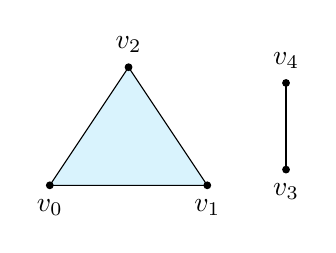
\begin{tikzpicture}
            \coordinate (a) at (0,0);
            \coordinate (b) at (2,0);
            \coordinate (c) at (1,1.5);
            \coordinate (d) at (3,.2);
            \coordinate (e) at (3,1.3);

            \filldraw[fill=cyan!15, draw=black] (a.center) -- (b.center) -- (c.center) -- cycle;

            \draw[black] (d) -- (e);

            \draw (a) node[circle,fill,inner sep=1pt,label=below:$v_0$]{};
            \draw (b) node[circle,fill,inner sep=1pt,label=below:$v_1$]{};
            \draw (c) node[circle,fill,inner sep=1pt,label=above:$v_2$]{};
            \draw (d) node[circle,fill,inner sep=1pt,label=below:$v_3$]{};
            \draw (e) node[circle,fill,inner sep=1pt,label=above:$v_4$]{};
        \end{tikzpicture}
    \end{center}
\end{remark}

\begin{definition}
    Let $K$ and $L$ be simplicial complexes. A function $f : V(K) \longrightarrow V(L)$ is a \emph{simplicial map}
    if for any simplex $\sigma = \{v_0, \dots, v_n\} \in K$, the images $\{f(v_0), \dots, f(v_n)\}$ is a simplex in $L$. That
    is, $f(\sigma) \in L$. A bijective simplicial map is a \emph{simplicial isomorphism}, and we say $K$ and $L$ are
    \emph{isomorphic}, $K \cong L$, if there is a simplicial isomorphism between them.
\end{definition}

\begin{remark}
    The collection of simplicial complexes together with simplicial maps forms the category $\mathbf{SCpx}$ of simplicial complexes.
    Note that even though we are only considering finite simplicial complexes, the collection of all simplicial complexes is a proper
    class.
\end{remark}

\begin{definition}
    A set $\sigma$ with $|\sigma| = n + 1$ is said to be an \emph{$n$-simplex}. The \emph{dimension} $\dim(K)$ of a simplicial
    complex $K$ is the maximum of the dimension of its simplices. The \emph{$n$-skeleton} $K^{(n)}$ of $K$ is the set of all
    $n$-simplices in $K$ (in particular $V(K) = K^{(0)}$), and the \emph{$c$-vector} of $K$ is the tuple $c_K \coloneqq
    (|K^{(0)}|, \dots, |K^{(\dim(K))}|)$. A simplicial complex $L \subseteq K$ is said to be a \emph{subcomplex}
    of $K$, and for a simplex $\sigma \in K$ we denote by $\bar{\sigma}$ the \emph{subcomplex generated by $\sigma$} (note
    that $\bar{\sigma} = \mathcal{P}(\sigma)$). For two simplices $\sigma, \tau \in K$ with $\tau \subseteq \sigma$, we say that
    $\tau$ is a \emph{face} of $\sigma$ and $\sigma$ is a \emph{coface} of $\tau$.
\end{definition}

\begin{definition}
    Let $K$ be a simplicial complex. Then $\sigma^{(n)}$ denotes an $n$-simplex in $K$, and write $\tau < \sigma^{(n)}$ to mean
    $\tau \subsetneq \sigma^{(n)}$; $\dim(\sigma) - \dim(\tau)$ is the \emph{codimension of $\tau$ with respect to $\sigma$}. The
    \emph{boundary} of a simplex $\sigma$ is $\partial_K(\sigma) \coloneqq \partial(\sigma) = \{\tau \in K^{(\dim(\sigma) - 1)}
    : \tau < \sigma\}$. A maximal simplex in $K$, that is, a simplex $\sigma$ which is not properly contained in any other simplex
    in $K$, is said to be a \emph{facet} of $K$.
\end{definition}

% \begin{proposition}
%     Let $K$ be a simplicial complex and let $\sigma$ be an $n$-simplex in $K$. Then $|\partial(\sigma)| = \dim(\sigma) + 1$.
% \end{proposition}
% \begin{proof}
%     Recall that $|\sigma| = n + 1$. Each face $\tau \in \partial(\sigma)$ is precisely a subset of $\sigma$ with
%     $|\tau| = |\sigma| - 1 = n$, of which there are $\binom{n+1}{n} = n+1 = \dim(\sigma) + 1$.
% \end{proof}

\begin{definition}
    Let $V$ be a finite set and $\mathcal{H} \subseteq \mathcal{P}(V) \setminus \{\varnothing\}$. The \emph{simplicial complex generated by
    $\mathcal{H}$}, denoted by $\langle \mathcal{H} \rangle$, is the smallest simplicial complex containing $\mathcal{H}$.
\end{definition}

% \begin{proposition}
%     If $\mathcal{H}$ is a simplicial complex then $\langle \mathcal{H} \rangle = \mathcal{H}$.
% \end{proposition}
% \begin{proof}
%     By definition, $\mathcal{H} \subseteq \langle \mathcal{H} \rangle$. Since $\mathcal{H}$ is a simplicial complex containing $\mathcal{H}$,
%     $\langle \mathcal{H} \rangle \subseteq \mathcal{H}$. Thus $\langle \mathcal{H} \rangle = \mathcal{H}$.
% \end{proof}

% \begin{proposition}
%     If $K$ is a simplicial complex and $\sigma \in K$, then $\bar{\sigma} = \langle \{\sigma\} \rangle$.
% \end{proposition}
% \begin{proof}
%     By definition, $\bar{\sigma} \subseteq \langle \{\sigma\} \rangle$, since $\langle \{\sigma\} \rangle$ is a simplicial complex which
%     contains $\sigma$. Similarly, $\bar{\sigma}$ is a simplicial complex containing $\sigma$, and hence $\langle \{\sigma\} \rangle
%     \subseteq \bar{\sigma}$. Thus $\bar{\sigma} = \langle \{\sigma\} \rangle$.
% \end{proof}

\subsection*{Some Examples.}

Let $V_n = \{v_0, \dots, v_n\}$ throughout.

\begin{example}
    We will (through some abuse of notation) denote by $0$ the \emph{trivial simplicial complex} $\langle \{V_0\} \rangle$.
    We may further abuse notation by identifying the simplicial complex $0$ with its point $0$.
\end{example}

\begin{example}
    The simplicial complex $\Delta^n \coloneqq \mathcal{P}(V_n) \setminus \{\varnothing\}$ is the (combinatorial)
    \emph{$n$-simplex}.

    The simplicial complex $\Delta S^n \coloneqq \Delta^{n+1} \setminus V_{n+1}$ is the \emph{simplicial $n$-sphere}. Its geometric
    realization is homeomorphic to the usual $n$-sphere $S^n$; it may be convenient to identify $\Delta S^n$ with $S^n$
\end{example}
    
\begin{example}
    Any simplicial complex $K$ of dimension 1 forms a \emph{graph} $(V(K), K^{(1)})$.
\end{example}

\begin{definition}
    Given a simplicial complex $K$, let $v \notin V(K)$ and define the \emph{cone over $K$} by
    \[
        \mathit{CK} \coloneqq K \cup \{v\} \cup \{\sigma \cup \{v\} : \sigma \in K\}.
    \]
\end{definition}

\begin{proposition}
    The cone over a simplicial complex $K$ is a simplicial complex.
\end{proposition}
\begin{proof}
    Let $\sigma \in \mathit{CK}$. We wish to show that any subset $\tau \subseteq \sigma$ is an element of $\mathit{CK}$. If $v \notin \sigma$, then
    $\sigma \in K$ and so $\tau \in K \subseteq \mathit{CK}$. If $v \in \sigma$, then let $\sigma' = \sigma \setminus \{v\} \in K$. If
    $v \notin \tau$, then $\tau \subseteq \sigma'$ and hence $\tau \in \mathit{CK}$. If $v \notin \tau$, then $\tau \setminus \{v\} \subseteq
    \sigma' \in K$, so $\tau \setminus \{v\} \in K$ and hence $\tau = (\tau \setminus \{v\}) \cup \{v\} \in \mathit{CK}$.
\end{proof}

\begin{example}
    As with the $n$-sphere, common topological spaces can be \emph{triangulated} and represented as simplicial complexes:
    \begin{figure}[H]
        \centering
        \begin{subfigure}{0.4\textwidth}
            \centering
            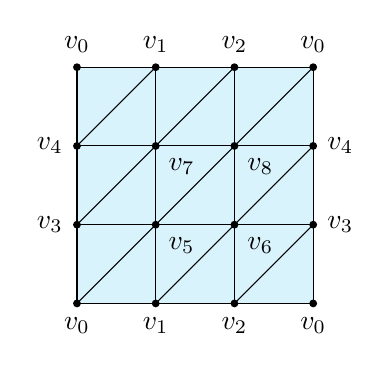
\begin{tikzpicture}[baseline=0]
                \filldraw[fill=cyan!15, draw=black] (0,0) -- (0,3) -- (3,3) -- (3,0) -- cycle;
                \draw (1,0) -- (1,3);
                \draw (2,0) -- (2,3);
                \draw (0,1) -- (3,1);
                \draw (0,2) -- (3,2);
                \draw (0,2) -- (1,3);
                \draw (0,1) -- (2,3);
                \draw (0,0) -- (3,3);
                \draw (1,0) -- (3,2);
                \draw (2,0) -- (3,1);
                \draw (0,0) node[circle,fill,inner sep=1pt,label=below:$v_0$]{};
                \draw (1,0) node[circle,fill,inner sep=1pt,label=below:$v_1$]{};
                \draw (2,0) node[circle,fill,inner sep=1pt,label=below:$v_2$]{};
                \draw (3,0) node[circle,fill,inner sep=1pt,label=below:$v_0$]{};
                \draw (0,1) node[circle,fill,inner sep=1pt,label=left:$v_3$]{};
                \draw (1,1) node[circle,fill,inner sep=1pt,label=below right:$v_5$]{};
                \draw (2,1) node[circle,fill,inner sep=1pt,label=below right:$v_6$]{};
                \draw (3,1) node[circle,fill,inner sep=1pt,label=right:$v_3$]{};
                \draw (0,2) node[circle,fill,inner sep=1pt,label=left:$v_4$]{};
                \draw (1,2) node[circle,fill,inner sep=1pt,label=below right:$v_7$]{};
                \draw (2,2) node[circle,fill,inner sep=1pt,label=below right:$v_8$]{};
                \draw (3,2) node[circle,fill,inner sep=1pt,label=right:$v_4$]{};
                \draw (0,3) node[circle,fill,inner sep=1pt,label=above:$v_0$]{};
                \draw (1,3) node[circle,fill,inner sep=1pt,label=above:$v_1$]{};
                \draw (2,3) node[circle,fill,inner sep=1pt,label=above:$v_2$]{};
                \draw (3,3) node[circle,fill,inner sep=1pt,label=above:$v_0$]{};
            \end{tikzpicture}
            \caption*{The torus $T^2$, $c_{T^2} = (9, 27, 18)$}
        \end{subfigure}
        \begin{subfigure}{0.4\textwidth}
            \centering
            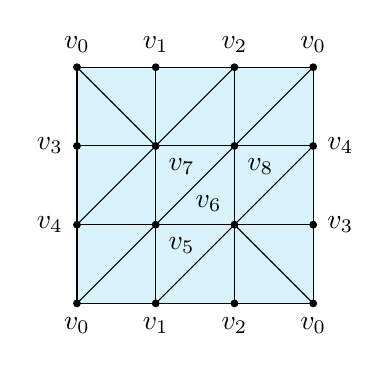
\begin{tikzpicture}[baseline=0]
                \filldraw[fill=cyan!15, draw=black] (0,0) -- (0,3) -- (3,3) -- (3,0) -- cycle;
                \draw (1,0) -- (1,3);
                \draw (2,0) -- (2,3);
                \draw (0,1) -- (3,1);
                \draw (0,2) -- (3,2);
                \draw (0,3) -- (1,2);
                \draw (0,1) -- (2,3);
                \draw (0,0) -- (3,3);
                \draw (1,0) -- (3,2);
                \draw (2,1) -- (3,0);
                \draw (0,0) node[circle,fill,inner sep=1pt,label=below:$v_0$]{};
                \draw (1,0) node[circle,fill,inner sep=1pt,label=below:$v_1$]{};
                \draw (2,0) node[circle,fill,inner sep=1pt,label=below:$v_2$]{};
                \draw (3,0) node[circle,fill,inner sep=1pt,label=below:$v_0$]{};
                \draw (0,1) node[circle,fill,inner sep=1pt,label=left:$v_4$]{};
                \draw (1,1) node[circle,fill,inner sep=1pt,label=below right:$v_5$]{};
                \draw (2,1) node[circle,fill,inner sep=1pt,label=above left:$v_6$]{};
                \draw (3,1) node[circle,fill,inner sep=1pt,label=right:$v_3$]{};
                \draw (0,2) node[circle,fill,inner sep=1pt,label=left:$v_3$]{};
                \draw (1,2) node[circle,fill,inner sep=1pt,label=below right:$v_7$]{};
                \draw (2,2) node[circle,fill,inner sep=1pt,label=below right:$v_8$]{};
                \draw (3,2) node[circle,fill,inner sep=1pt,label=right:$v_4$]{};
                \draw (0,3) node[circle,fill,inner sep=1pt,label=above:$v_0$]{};
                \draw (1,3) node[circle,fill,inner sep=1pt,label=above:$v_1$]{};
                \draw (2,3) node[circle,fill,inner sep=1pt,label=above:$v_2$]{};
                \draw (3,3) node[circle,fill,inner sep=1pt,label=above:$v_0$]{};
            \end{tikzpicture}
            \caption*{The Klein bottle $\mathcal{K}$, $c_\mathcal{K} = (9, 27, 18)$}
        \end{subfigure}
    \end{figure}
\end{example}

\begin{definition}
    Let $K$ be a simplicial complex and let $n = \dim(K)$, and put $c_i = |K^{(i)}|$.
    The \emph{Euler characteristic} $\chi(K)$ of $K$ is given by
    \[
        \chi(K) = \sum_{i=0}^n (-1)^i c_i(K).
    \]
\end{definition}

\subsubsection*{An aside on CW complexes.}

Simplicial complexes are generalized by the idea of CW complexes, a standard concept in algebraic topology.

\begin{definition}
    An \emph{$n$-cell} is a copy of an $n$-dimensional disc $D^n$.
\end{definition}

\begin{definition}
    A \emph{CW complex} is a topological space $X$ defined as follows:
    \begin{enumerate}
        \item Let $X^0$ be a discrete set whose points are regarded as 0-cells.
        \item Inductively define the \emph{n-skeleton} $X^n$ from $X^{n-1}$ by attatching $n$-cells $e^n_\alpha$
        according to maps $\varphi_\alpha : S^{n-1} \to X^{n-1}$ so that $X^n$ is a quotient of $X^{n-1} \bigsqcup_\alpha D_\alpha^n$
        under $x \sim \varphi_\alpha(x)$ for $x \in \partial D_\alpha^n$.
        \item Continue until some finite $n \in \N$ and let $X = X^n$; or continue and put $X = \bigcup_n X^n$ endowed with the weak topology:
        $A \subseteq X$ is open if and only if $A \cap X^n$ is open in $X^n$ for each $n$.
    \end{enumerate}
    If $X = X^n$ for some $n$, then $X$ is said to be \emph{finite-dimensional}, and its dimension is $n$
    \footnote{These standard definitions can be found in texts such as Hatcher's \emph{Algebraic Topology}.}.
\end{definition}

\begin{remark}
    Note that (the geometric realization of) a simplicial complex is a CW complex.
\end{remark}

\subsection{Simple Homotopy.}

\begin{definition}
    Let $K$ be a simplicial complex and suppose we have $\sigma^{(d-1)} < \tau^{(d)} \in K$ such that $\tau$ is the only coface
    of $\sigma$. Then the simplicial complex $K \setminus \{\sigma, \tau\}$ is an \emph{elementary collapse} of $K$, denoted by
    $K \searrow K \setminus \{\sigma, \tau\}$. Now suppose $\sigma^{(d-1)} < \tau^{(d)} \notin K$, where every other face of
    $\tau$ is in $K$. Then $K \nearrow K \cup \{\sigma, \tau\}$ in an \emph{elementary expansion} of $K$. The pair $\{\sigma,
    \tau\}$ is a \emph{free pair} of simplices. Two simplicial complexes $K$ and $L$ are said to be \emph{simple homotopy
    equivalent} or of the same $\emph{simple homotopy type}$, denoted $K \wedgearrow L$ if there is a series of elementary
    collapses and expansions from $K$ to $L$. If $K \wedgearrow 0$, $K$ is said to have the \emph{simple homotopy type of a
    point}.
\end{definition}

\begin{remark}
    This is a refinement of the typical notion of homotopy equivalence.
    \footnote{More details (and generality) can be found in Marshall M. Cohen's \textit{A Course in Simple-Homotopy Theory}.}
\end{remark}

\begin{example}
    We can communicate the a sequence of collapses from one simplicial complex to another by decorating it with arrows:
    \begin{center}
        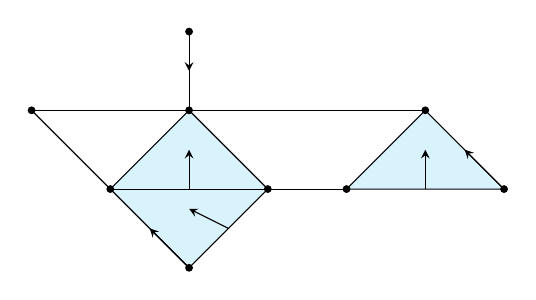
\begin{tikzpicture}
            \filldraw[fill=cyan!15, draw=black] (1,-1) -- (2,-2) -- (3,-1) -- (2, 0) -- cycle;
            \filldraw[fill=cyan!15, draw=black] (4,-1) -- (5, 0) -- (6,-1) -- cycle;
            \draw (0, 0) -- (1,-1);
            \draw (0, 0) -- (5, 0);
            \draw (2, 1) -- (2, 0);
            \draw (1,-1) -- (4,-1);
            \draw (0, 0) node[circle,fill,inner sep=1pt]{};
            \draw (1,-1) node[circle,fill,inner sep=1pt]{};
            \draw (2, 0) node[circle,fill,inner sep=1pt]{};
            \draw (2, 1) node[circle,fill,inner sep=1pt]{};
            \draw (2,-2) node[circle,fill,inner sep=1pt]{};
            \draw (3,-1) node[circle,fill,inner sep=1pt]{};
            \draw (4,-1) node[circle,fill,inner sep=1pt]{};
            \draw (5, 0) node[circle,fill,inner sep=1pt]{};
            \draw (6,-1) node[circle,fill,inner sep=1pt]{};

            \draw[-stealth] (2, 1) -- (2, .5);
            \draw[-stealth] (2,-1) -- (2,-.5);
            \draw[-stealth] (2,-2) -- (1.5,-1.5);
            \draw[-stealth] (2.5,-1.5) -- (2,-1.25);
            \draw[-stealth] (5,-1) -- (5,-.5);
            \draw[-stealth] (6,-1) -- (5.5,-.5);
        \end{tikzpicture}
    \end{center}
\end{example}

\begin{proposition}
    Let $\{\sigma, \tau\}$ be a free pair of a simplicial complex $K$. Then $K \setminus \{\sigma, \tau\}$ is a simplicial complex.
\end{proposition}
\begin{proof}
    Since $\tau$ is the only coface of $\sigma$, it must be that $\tau$ is a facet of $K$ (for otherwise $\sigma$ would have another
    coface), so we may remove $\tau$; we may also remove $\sigma$ because $\tau$ is the only coface of $\sigma$, so $\sigma$ is a facet
    of $K \setminus \{\tau\}$, hence $K \setminus \{\sigma, \tau\}$ is a simplicial complex.
\end{proof}

\begin{proposition}
    Simple homotopy equivalence of simplicial complexes is an equivalence relation.
\end{proposition}
\begin{proof}
    Let $K$ be a simplicial complex. Of course $K$ is simple homotopy equivalent to itself, since doing no collapses or expansions
    preserves $K$. Now let $L$ be a simplicial complex and $K \wedgearrow L$. Then each elementary collapse can be
    undone by an elementary expansion and vice versa, so $L \wedgearrow K$. Finally, let $H$ be a simplicial complex
    and suppose $K \wedgearrow L$ and $L \wedgearrow H$. Then there is a series of elementary collapses from $K$
    to $L$, and from $L$ to $H$, so simply concatenating these yields a series of elementary collapses
    and expansions from $K$ to $H$. Hence $K \wedgearrow H$ and so simple homotopy equivalence is an equivalence
    relation.
\end{proof}

\begin{definition}
    A property $\alpha(K)$ of a simplicial complex $K$ is a \emph{simple homotopy invariant} if for any $L \wedgearrow K$,
    we have $\alpha(L) = \alpha(K)$.
\end{definition}

\begin{proposition}
    The Euler characteristic $\chi(K)$ is a simple homotopy invariant.
\end{proposition}
\begin{proof}
    Let $\{\sigma^{(d-1)}, \tau^{(d)}\}$ be a free pair in $K$ and let $K' = K \setminus \{\sigma, \tau\}$. Then if $c_K = (c_0, \dots, c_n)$
    then the elementary collapse $K \searrow K'$ has $c_\{K'\} = (c_0, \dots, c_{d-1} - 1, c_d - 1, \dots, c_n)$ so $\chi(K') = \chi(K) +
    (-1)^{d-1} + (-1)^d = \chi(K) + 1 - 1 = \chi(K)$. Similarly, if $K'$ is the result of an elementary expansion then $\chi(K') = \chi(K)$.
    By induction, $\chi(K)$ is invariant under any finite number of elementary collapses and expansions, so $\chi$ is a simple homotopy invariant.
\end{proof}

\begin{definition}
    A simplicial complex $K$ is \emph{collapsible} if there is a sequence of elementary collapses
    \[
        K = K_0 \searrow \dots \searrow K_n = 0.  
    \]
\end{definition}

\begin{definition}
    Let $K$ and $L$ be (disjoint) simplicial complexes. Their \emph{join} $K * L$ is the simplicial complex
    \[
        K * L \coloneqq K \sqcup \mathcal L \sqcup \{\sigma \sqcup \tau : \sigma \in K, \tau \in L\}.
    \]
\end{definition}

\begin{remark}
    The cone over $K$ is a special case of a join: $\mathit{CK} \cong K * 0$.
\end{remark}

\begin{definition}
    Let $v, w \notin K$, $v \neq w$. The \emph{suspension} of a simplicial complex $K$ is defined by $\Sigma K \coloneqq K * \{v,w\}$.
\end{definition}

% \begin{proposition}
%     Let $\sigma$ be a facet of a simplicial complex $K$. Let $\mathit{CK} = K * \{v\}$.
%     Then $\mathit{CK} \setminus \{\sigma, \sigma \cup \{v\}\} = C(K \setminus \{\sigma\})$.
% \end{proposition}
% \begin{proof}
%     \begin{align*}
%         \mathit{CK} \setminus \{\sigma, \sigma \cup \{v\}\} &= (K * \{v\}) \setminus \{\sigma, \sigma \cup \{v\}\} \\
%             &= (K \cup \{v\} \cup \{\tau \cup \{v\} : \tau \in K\}) \setminus \{\sigma, \sigma \cup \{v\}\} \\
%             &= (K \setminus \{\sigma\}) \cup \{v\} \cup \{\tau \cup \{v\} : \tau \in (K \setminus \{\sigma\})\} \\
%             &= (K \setminus \{\sigma\}) * \{v\} \\
%             &= C(K \setminus \{\sigma\})
%     \end{align*}
% \end{proof}

% \begin{proposition}
%     The cone over any simplicial complex is collapsible.
% \end{proposition}
% \begin{proof}
%     By induction on $n = |K|$. Of course for $n = 0$, $\mathit{CK} = C0$ is collapsible. Now suppose that for some $n \geq 1$, any cone over $n$
%     simplices is collapsible. Then let $K$ be a simplicial complex with $n+1$ simplices, and consider $\mathit{CK} = K * \{v\}$. Notice that if
%     $\sigma$ is a facet of $K$ then $\{\sigma, \sigma \cup \{v\}\}$ is a free pair in $\mathit{CK}$, so $\mathit{CK} \searrow \mathit{CK} \setminus
%     \{\sigma, \sigma \cup \{v\}\}$. But $\mathit{CK} \setminus \{\sigma, \sigma \cup \{v\}\} = C(K \setminus \{\sigma\})$ is a cone over $n$ simplices
%     and hence is contractible by the inductive hypothesis. Thus $\mathit{CK} \searrow C(K \setminus \{\sigma\}) \searrow 0$ so by induction every cone
%     is collapsible.
% \end{proof}

% \begin{proposition}
%     If $K \searrow H$ and $H \searrow L$, then $K \wedgearrow H \wedgearrow L$.
% \end{proposition}
% \begin{proof}
%     Simple homotopy involves expansions and collapses.
% \end{proof}

\begin{remark}
    There exist simplicial complexes with the simple homotopy type of a point but are not collapsible, one example being the \emph{dunce hat}
    complex\autocite{duncehat}.
\end{remark}

\section{Discrete Morse Theory.}

Morse theory is tool in differential topology that allows one to study the topology of a smooth manifold $M$ by studying smooth functions
$f \in C^\infty(M, \R)$, and in particular their (non-degenerate) critical points\autocite{morsetheory}. The discrete theory allows us to use
similar techniques to study simplicial complexes by abstracting the idea of critical points to a discrete object.

\subsection{Discrete Morse Functions.}

\subsubsection{Basic Discrete Morse Functions.}

The following notion is due to Bruno Benedetti:

\begin{definition}
    Let $K$ be a simplicial complex. A function $f : K \to \R$ is \emph{weakly increasing} if for each $\sigma \subseteq \tau \in K$ we have
    $f(\sigma) \leq f(\tau)$. A \emph{basic discrete Morse function} is a weakly increasing function which is at most 2-to-1 (i.e. for each
    $x \in \R$, $|f^{-1}(x)| \leq 2$) and if $f(\sigma) = f(\tau)$ then either $\sigma \subseteq \tau$ or $\tau \subseteq \sigma$.  
\end{definition}

\begin{definition}
    Given a basic discrete Morse function $f : K \to \R$, a simplex $\sigma \in K$ is \emph{critical} if $f$ is injective on $\sigma$,
    and the value $f(\sigma)$ is a \emph{critical value} of $f$. Otherwise $\sigma$ is \emph{regular} and $f(\sigma)$ is a \emph{regular value}.
\end{definition}

\subsubsection{Discrete Morse Functions.}

The usual definition for CW complexes is due to Robin Forman\autocite{morsecells}:
\begin{definition}
    Let $X$ be a CW complex and $\mathcal{X}$ its set of cells. A function $f : \mathcal{X} \to \R$ is a \emph{discrete Morse function} if:
    \begin{enumerate}
        \item For any cell $\sigma \in \mathcal{X}$, the number of cells $\tau \in \mathcal{X}$ in the boundary of $\sigma$ which satisfy
        $f(\sigma) \leq f(\tau)$ is at most one.
        \item For any cell $\sigma \in \mathcal{X}$, the number of cells $\tau \in \mathcal{X}$ containing $\sigma$ in their boundary which satisfy
        $f(\sigma) \geq f(\tau)$ is at most one.
    \end{enumerate}
\end{definition}

We present the definition here, as Scofield does, for simplicial complexes:

\begin{definition}
    A function $f : K \to \R$ is a \emph{discrete Morse function} if for every $n$-simplex $\sigma \in K$,
    \begin{align*}
        |\{\tau^{n-1} < \sigma : f(\tau) \geq f(\sigma)\}| &\leq 1 \\
        |\{\tau^{n+1} > \sigma : f(\tau) \leq f(\sigma)\}| &\leq 1.
    \end{align*}
\end{definition}
That is, any simplex $\sigma$, has at most one face $\tau$ with $f(\tau) \geq f(\sigma)$ and any $\sigma \in K$ has at most one coface
$\tau$ with $ f(\tau) \leq f(\sigma)$.

\begin{remark}
    In the continuous theory, a Morse function $f : M \to \R$ is a smooth function with no degenerate critical points.

    The idea of a critical point in this setting is not dissimilar from the familiar concept in multivariable calculus: let $p \in M$ and let
    $U \subseteq M$ be an open neighborhood of $p$ with a local coordinate chart $(x^1, \dots, x^n)$. Then $p$ is a critical point if
    \[
        \frac{\partial f}{\partial x^1}(p) = \dots = \frac{\partial f}{\partial x^n}(p) = 0
    \]
    and $f(p)$ is said to be a critical value of $f$.

    This does not depend on the coordinate system: given a differentiable map $\varphi : M \to N$ of smooth manifolds and a point $p \in M$,
    the differential (or pushforward) $\varphi_* : TM_p \to TN_{\varphi(p)}$ (or $\text{d}\varphi_p$) is a linear map between the tangent spaces
    of $M$ at $p$ and $N$ at $\varphi(p)$. If particular, with $f : M \to \R$, let $f_* : TM_p \to T\R_{f(p)}$ be the induced linear map of tangent spaces.
    In this setting, a point $p \in M$ is a critical point of $f$ if $f_*(p) = 0$.

    The non-degeneracy condition is similar: using the same local coordinate chart, the critical point $p$ is non-degenerate if and oly if the matrix
    \[
        \left(\mathbf{H}_f(x)\right)_{i,j} = \left(\frac{\partial^2 f}{\partial x^i \partial x^j}\right)_{i,j}
    \]
    is non-singular (the intrinsic definition of the Hessian $f_{**}$ is more involved, but can be found in Milnor\autocite*{morsetheory}).
\end{remark}



\end{document}